\documentclass[aspectratio=43]{beamer}
\usepackage[utf8]{inputenc}

%%%%%%%%%%%%%%%%%%%%%%%% THEME
\usetheme{material}
\useLightTheme
\usePrimaryDeepOrange
\useAccentCyan

\usepackage{macros} % must come after theme

\title{\qis}
\keywords{\qis}

\begin{document}

\begin{frame}
	\titlepage
\end{frame}


\begin{frame}{Table of contents}
	\begin{card}
		\tableofcontents
	\end{card}
\end{frame}


\section{Introduction}
\begin{frame}{Introduction}
    \begin{card}
    This week we are going to build the bridge between \textbf{\qm} and \textbf{\qc}, in other words, how the \q laws can be leveraged into the tools we need for, well, computing! This will be done through a parallelism with \cc. \\
    Furthermore, we will also go through our first \textbf{\qk snippets} and finish of by running our first \q circuit on a \textbf{real Quantum Processor}, using \ibmqe. \qasm language will also be briefly mentioned as a tool for this course. 
    \end{card}
\pagenumber
\end{frame}

\section{\qis}
\begin{frame}{\qis}
    \begin{card}
    Is a broad area of studies, it is the \q sibling of typical information science. It is concerned with \textbf{representing}, \textbf{manipulating} and \textbf{maintaining} information in quantum states. It tackles many problems that did not exist, at least in the same form, in \cc, such as \textit{quantum error correction}, \textit{quantum teleportation}, \textit{quantum communication}, ...
    \end{card}
\pagenumber
\end{frame}

\section{Classical bits}
\begin{frame}{Classical bits}
    \begin{card}
    The simplest unit of information in classical systems, a bit (short for binary unit), which can store either a 0 or a 1 value, thus binary. 
    \end{card}
    \begin{card}
    There is quite an interesting metaphor for explaining the difference between bits and their quantum equivalent, based on the concept of coin tossing, from which we will start!
    \end{card}
\pagenumber
\end{frame}

\begin{frame}{Coin tossing for bits}
	\begin{multicols}{2}
		[
		\begin{cardTiny}
			When you toss a coin, the result will either be tails or heads - 0 or 1 (please try not to think of the cases of a vertical landing until you can do it). This is a binary and deterministic state.
		\end{cardTiny}
		]
        \begin{center}
	        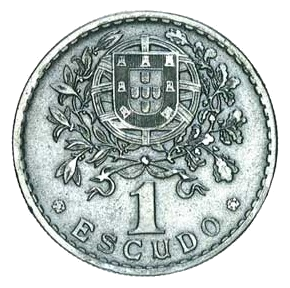
\includegraphics[width=0.2\textwidth]{escudo_tails}
	        \\Tails = 0
    	\end{center}
        \begin{center}
	        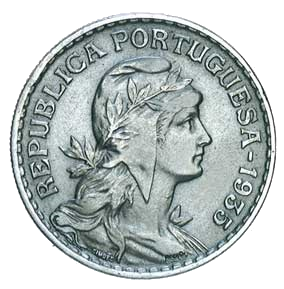
\includegraphics[width=0.2\textwidth]{escudo_heads}
	        \\Heads = 1
    	\end{center}
	\end{multicols}
	\begin{cardTiny}
		\textbf{classical register:} is an array of n independent bits. A 1-bit register is simply a bit and can be in 1 out of $2^1 = 2$ possible states, whereas an 8-bit register can be in 1 out of $2^8 = 256$ states.
	\end{cardTiny}
\pagenumber
\end{frame}

\section{\q bits}
\subsection{qubits}
% https://twitter.com/drtaliagershon?lang=en
% include qiskit snippets of both code parts
\begin{frame}{qubit}
    \begin{card}
    Assuming you have a quantum state (isolated from interference) that has not been measured. If we refer back to the 2 possible states from Week 0, we know our state is a combination of both 0 and 1, remember? \begin{equation*}
        \superpos
    \end{equation*}
    But what does this mean, exactly? Well, that our system is not in just one of the states (assuming $\alpha \neq 0 \wedge \beta \neq 0$), it holds the information of both possible states, at the same time.
    \end{card}
\pagenumber
\end{frame}

\begin{frame}{Coin tossing for qubits}
    \begin{card}
        And so, instead of heads or tails, we can compare this state to a coin that is still spinning. Such is the essence of the qubit, a simultaneous state of 0 and 1 (described according to the probability distribution of $\alpha$ and $\beta$).  Notice that the state is not hidden according to the probabilities, but rather comprised of both possibilities!  
    \end{card}
    \begin{center}
        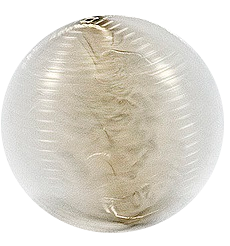
\includegraphics[width=0.2\textwidth]{spinning_coin}
        \\$\superpos$
    \end{center}
\pagenumber
\end{frame}

\begin{frame}{qubit}
    \begin{card}
        Unlike a bit, we now have a single quantum state with two simultaneous states. Why does this matter? Because this uncertainty contains in itself much more than a deterministic bit, so that when we perform operations, they are applied to all possible states and not just the one.
    \end{card}
	\begin{cardTiny}
		\textbf{\q register:} is an array of n qubits. A 1-bit quantum register is simply a qubit and can hold $2^1 = 2$ possible states, whereas an 8-qubit quantum register can hold $2^8 = 256$ states, not just 1 of them like classical registers, all of them!!
	\end{cardTiny}
\pagenumber
\end{frame}

\begin{frame}{Coin tossing metaphor}
	\begin{cardTiny}
		If we have one coin, the state \textbf{can be} 0 or 1.
	\end{cardTiny}
    \begin{center}
        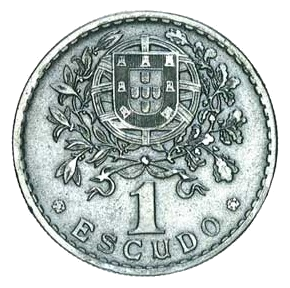
\includegraphics[width=0.2\textwidth]{escudo_tails}\\
        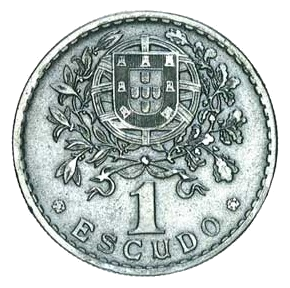
\includegraphics[width=0.1\textwidth]{escudo_tails}
        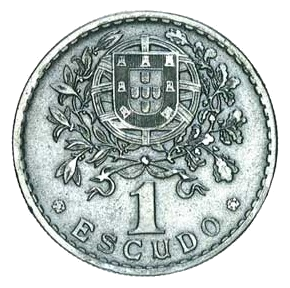
\includegraphics[width=0.1\textwidth]{escudo_tails}\\
        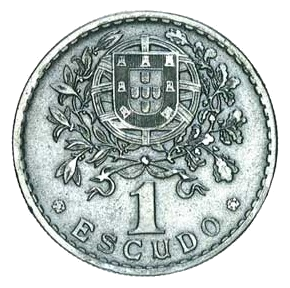
\includegraphics[width=0.1\textwidth]{escudo_tails}
        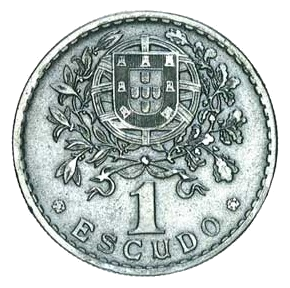
\includegraphics[width=0.1\textwidth]{escudo_tails}
        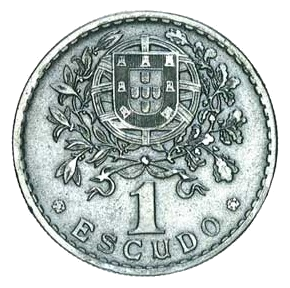
\includegraphics[width=0.1\textwidth]{escudo_tails}\\...
	\end{center}
\pagenumber
\end{frame}

\begin{frame}{Coin tossing metaphor}
	\begin{cardTiny}
		If we have two coins,the state \textbf{can be} 00 or 01 or 10 or 11. 
	\end{cardTiny}
    \begin{center}
        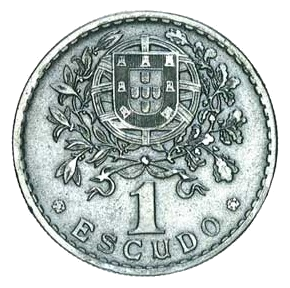
\includegraphics[width=0.1\textwidth]{escudo_tails}\\
        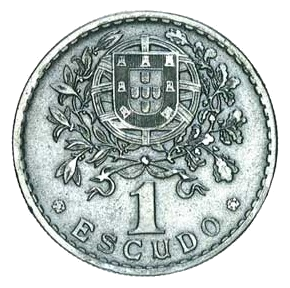
\includegraphics[width=0.2\textwidth]{escudo_tails}
        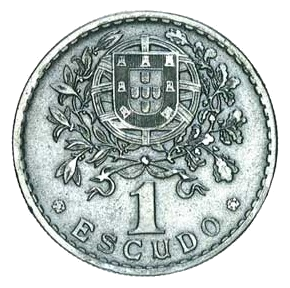
\includegraphics[width=0.2\textwidth]{escudo_tails}\\
        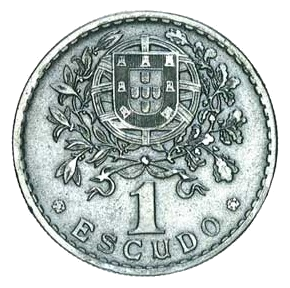
\includegraphics[width=0.1\textwidth]{escudo_tails}
        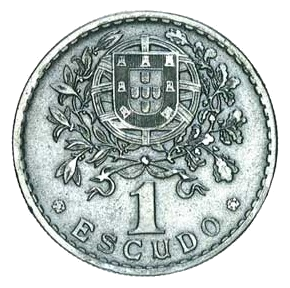
\includegraphics[width=0.1\textwidth]{escudo_tails}
        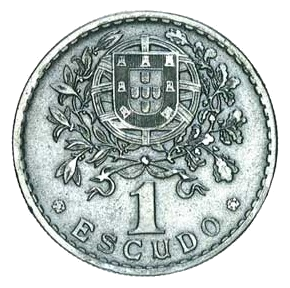
\includegraphics[width=0.1\textwidth]{escudo_tails}\\...
	\end{center}
\pagenumber
\end{frame}

\begin{frame}{Coin tossing metaphor}
	\begin{cardTiny}
		If we have three coins,the state \textbf{can be} 000 or 001 or 010 or 011 or 100 or 101 or 110 or 111. 
	\end{cardTiny}
    \begin{center}
        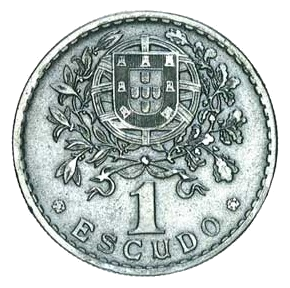
\includegraphics[width=0.1\textwidth]{escudo_tails}\\
        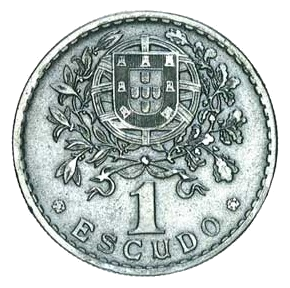
\includegraphics[width=0.1\textwidth]{escudo_tails}
        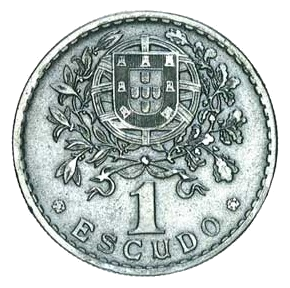
\includegraphics[width=0.1\textwidth]{escudo_tails}\\
        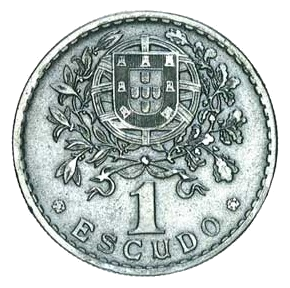
\includegraphics[width=0.2\textwidth]{escudo_tails}
        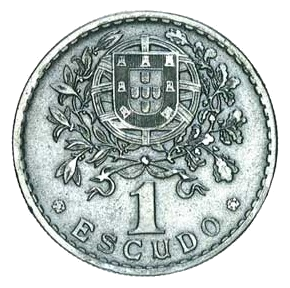
\includegraphics[width=0.2\textwidth]{escudo_tails}
        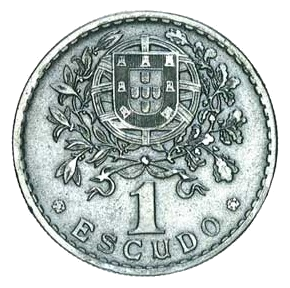
\includegraphics[width=0.2\textwidth]{escudo_tails}\\...
	\end{center}
\pagenumber
\end{frame}

\begin{frame}{Coin tossing metaphor}
	\begin{card}
		Essentially if we have \textbf{n} coins, we can have 1 of the \textbf{$2^n$} possible states.\\
		For n=4 ($2^4=16$ possible states), 1010 would be:
	\end{card}
    \begin{center}
        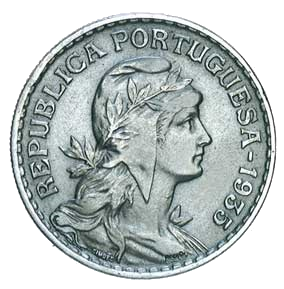
\includegraphics[width=0.2\textwidth]{escudo_heads}
        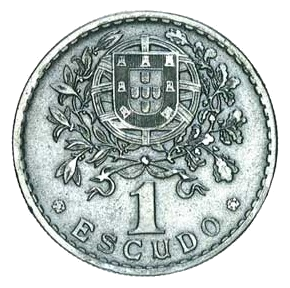
\includegraphics[width=0.2\textwidth]{escudo_tails}
        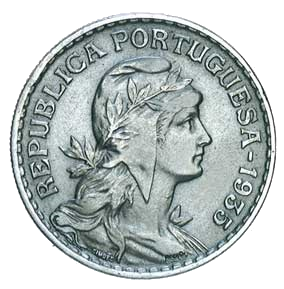
\includegraphics[width=0.2\textwidth]{escudo_heads}
        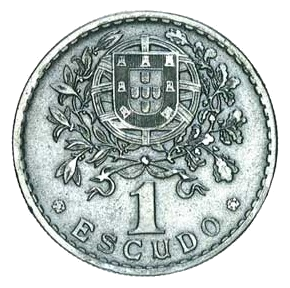
\includegraphics[width=0.2\textwidth]{escudo_tails}
	\end{center}
\pagenumber
\end{frame}

%%%%%Qubit coins
\begin{frame}{Coin tossing metaphor}
	\begin{cardTiny}
		If we have one spinning coin, the state \textbf{is} 0 and 1.
	\end{cardTiny}
    \begin{center}
        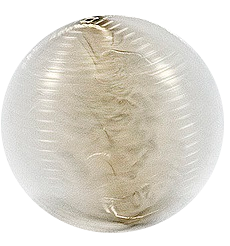
\includegraphics[width=0.2\textwidth]{spinning_coin}\\
        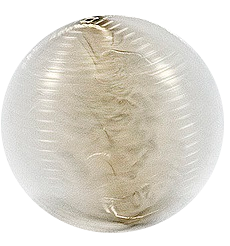
\includegraphics[width=0.1\textwidth]{spinning_coin}
        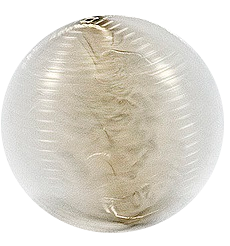
\includegraphics[width=0.1\textwidth]{spinning_coin}\\
        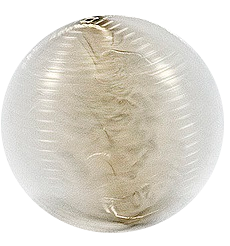
\includegraphics[width=0.1\textwidth]{spinning_coin}
        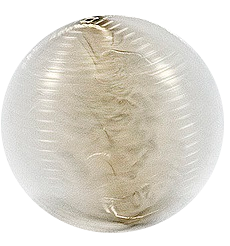
\includegraphics[width=0.1\textwidth]{spinning_coin}
        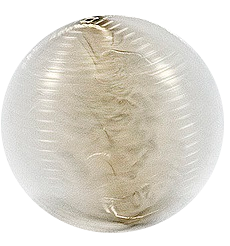
\includegraphics[width=0.1\textwidth]{spinning_coin}\\...
	\end{center}
\pagenumber
\end{frame}

\begin{frame}{Coin tossing metaphor}
	\begin{cardTiny}
		If we have two (independent) spinning coins, the state \textbf{is} 00 and 01 and 10 and 11.
	\end{cardTiny}
    \begin{center}
        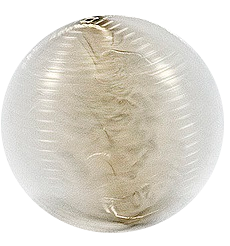
\includegraphics[width=0.1\textwidth]{spinning_coin}\\
        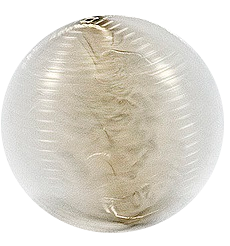
\includegraphics[width=0.2\textwidth]{spinning_coin}
        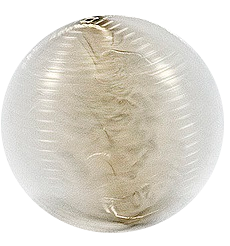
\includegraphics[width=0.2\textwidth]{spinning_coin}\\
        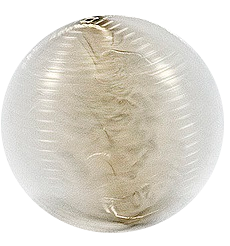
\includegraphics[width=0.1\textwidth]{spinning_coin}
        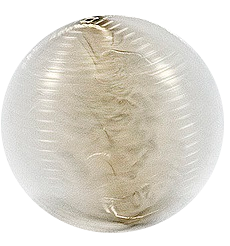
\includegraphics[width=0.1\textwidth]{spinning_coin}
        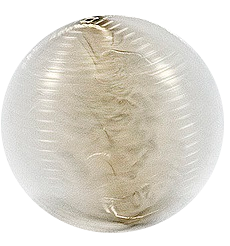
\includegraphics[width=0.1\textwidth]{spinning_coin}\\...
	\end{center}
\pagenumber
\end{frame}

\begin{frame}{Coin tossing metaphor}
	\begin{cardTiny}
		If we have three (independent) spinning coins, the state \textbf{is} 000 and 001 and 010 and 011 and 100 and 101 and 110 and 111. 
	\end{cardTiny}
    \begin{center}
        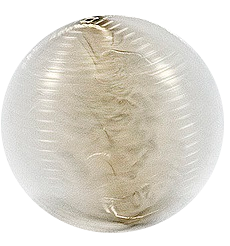
\includegraphics[width=0.1\textwidth]{spinning_coin}\\
        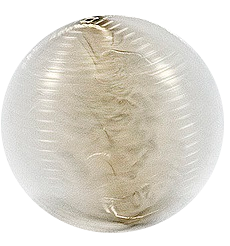
\includegraphics[width=0.1\textwidth]{spinning_coin}
        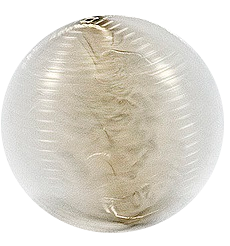
\includegraphics[width=0.1\textwidth]{spinning_coin}\\
        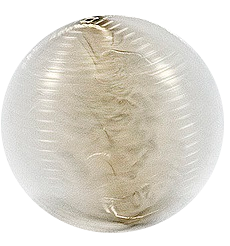
\includegraphics[width=0.2\textwidth]{spinning_coin}
        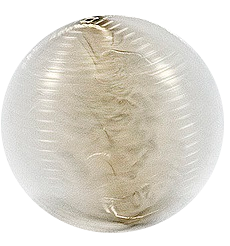
\includegraphics[width=0.2\textwidth]{spinning_coin}
        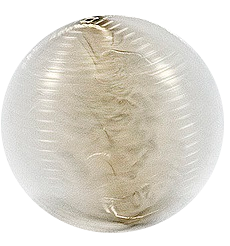
\includegraphics[width=0.2\textwidth]{spinning_coin}\\...
	\end{center}
\pagenumber
\end{frame}

\begin{frame}{Coin tossing metaphor}
	\begin{card}
		Essentially if we have \textbf{n} (independent) spinning coins, we can have  \textbf{$2^n$} possible states simultaneously.\\
		For $n=4$ our state holds $2^4=16$ possibilities. The information we can have grows \textbf{exponentially} with the number of spinning coins or, let me unveil the curtain, qubits! Such is the power of the qubit, and this "supercharged" version of the bit will help us understand why \qc really tips the scales.
	\end{card}
\pagenumber
\end{frame}

\subsection{qudits}
\begin{frame}{qudits}
    \begin{card}[Curiosity*]
        As the bits also have higher order units (\href{https://en.wikipedia.org/wiki/Ternary_numeral_system}{trit} for a ternary state, ...) so does the qubit have its d-order equivalent: the \textbf{qudit} (quantum d-git).\\
        For the initial case of the hydrogen atom, we could simply consider it as having 3 possible orbits, thus $\ket{0}$, $\ket{1}$ and $\ket{2}$ (a qudit with $d=3$ is actually a qutrit - quantum trit).\\
        Nevertheless, we will not spend much time with these units as their use is not so straightforward, and once you master qubits, it is easier to extrapolate to other arities than the other way around!
    \end{card}
\pagenumber
\end{frame}

\section{Hands-on}
\begin{frame}[fragile]{Hands-on - Registers}
Let us now write some python that will follow us through many lessons to come.\\
Here's how to create a \href{https://qiskit.org/documentation/_autodoc/qiskit._classicalregister.html?highlight=classicalregister#module-qiskit._classicalregister}{ClassicalRegister} on \qk:
\begin{cardTiny}
\begin{minted}{python}
from qiskit import ClassicalRegister
# Create a Classical Register with 2 bits.
c = ClassicalRegister(2)
\end{minted}
\end{cardTiny}
%%%%%%%
Likewise for \href{https://qiskit.org/documentation/_autodoc/qiskit._quantumregister.html?highlight=quantumregister#module-qiskit._quantumregister}{QuantumRegister}:
\begin{cardTiny}
\begin{minted}{python}
from qiskit import QuantumRegister
# Create a Quantum Register with 2 qubits.
q = QuantumRegister(2)
\end{minted}
\end{cardTiny}
For our purpose, classical registers will serve only to save the results of measurements on qubits.
\end{frame}

\begin{frame}[fragile]{Hands-on - Quantum Circuit}
To connect our classical and quantum registers in a \href{https://qiskit.org/documentation/_autodoc/qiskit._quantumcircuit.html#qiskit._quantumcircuit.QuantumCircuit}{QuantumCircuit} we do:
\begin{cardTiny}
\begin{minted}{python}
from qiskit import QuantumCircuit
# Create a Quantum Circuit
qc = QuantumCircuit(q, c)
# perform a measurement of our qubits into our bits
qc.measure(q, c)
\end{minted}
\end{cardTiny}
What we can do so far is quite limited, but these are the building blocks we need. In the next lesson we will take a look at the operations that can happen before we measure a quantum circuit!
\end{frame}


\begin{frame}[fragile]{Hands-on - Quantum Circuit Visualization}
Here is the code for visualizing our mighty complex circuit:
\begin{cardTiny}
\begin{minted}{python}
from qiskit.tools.visualization 
 import matplotlib_circuit_drawer as draw
draw(qc) # visualize our quantum circuit
\end{minted}
\end{cardTiny}
\begin{center}
    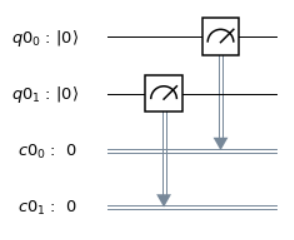
\includegraphics[width=0.25\textwidth]{circuit_01_measurement}
\end{center}
\small{
    You will notice that both qubits ($q0_0$ and $q0_1$) are initially in state $\ket{0}$ meaning that $\beta=0$ in $\superpos$ (what do you think $\alpha=$?). This is by design and how most experiments begin. The symbol connecting the qubit to each bit is the universal symbol for quantum measurement.
}
\end{frame}

\section{\qasm}
\begin{frame}[fragile]{\qasm}
    \begin{cardTiny}
    \small{
    \qasm derives from `Open Quantum Assembly Language' and reads `kazm'. This is a rather recent invention, coming of of a \href{https://arxiv.org/abs/1707.03429}{2017 paper}. It is a descriptive language that maps a quantum circuit as text instructions. It has since became a standard and, although we will not be going deeper into it, it is good to understand the overall structure of these documents, here is the example for the above circuit (q0 was changed into q, and c0 to c due to some \qasm interpreters):
    }
    \end{cardTiny}
    \begin{cardTiny}
    \begin{minted}{vhdl} % since qasm is not yet supported
OPENQASM 2.0;
include "qelib1.inc";
qreg q[2];
creg c[2];
x q[0];
measure q[0] -> c[0];
measure q[1] -> c[1];
    \end{minted}
    \end{cardTiny}
\end{frame}
%https://quantumexperience.ng.bluemix.net/qx/editor

\begin{frame}[fragile]{QASM + \ibmqe exercise}
\small{
    \href{https://quantumexperience.ng.bluemix.net/qx/experience}{\ibmqe} supports QASM in their online editor, and you can literally use a GUI and check the \qasm equivalent (and vice versa).  Your task is to go to the \href{https://quantumexperience.ng.bluemix.net/qx/editor}{editor} and do the following:
    \begin{itemize}
        \itemsep0em 
        \item Login into \ibmqe
        \item Click on "New" for a new experiment
        \item Name it as you like (eg. "qasm\_test")
        \item Choose ibmqx2 or ibmqx4 (look for available)
        \item Click on "Switch to \qasm editor"
        \item Paste the above \qasm code and see the visual result
        \item Press "Simulate" and see the result (should be $00$ with $1.000$ frequency, this means that out of all the repetitions of the experiment, $100\%$ resulted in $00$).
        \item Go ahead and press "Run" and, just for this once, ignore if there is a cached version and choose "New Execution"!
    \end{itemize}
    You just executed instructions on a \q Computer, you will receive an email with the results (may be more queued jobs ahead of you).
}
\end{frame}

\begin{frame}{\qk exercise}
    \begin{card}
    The code provided here has been written to a \href{\weekTwo/exercises/w2_01.ipynb}{Jupyter Notebook} that you are encouraged to execute on your machine, as that exercise will help you understand \qk from the beginning. There is also a code sample for generating the \qasm instructions and, at the end of the notebook, there are more suggested exercises. This, along with the previous slide on testing \ibmqe are your tasks for the week. Feel free, of course, to take some extra steps and trying out new stuff on your version of the notebook!
    \end{card}
\pagenumber
\end{frame}



% \section{Computational Complexity}
% % https://en.wikipedia.org/wiki/BQP
% % https://www.quantiki.org/wiki/bqp
% \begin{frame}{Frame Title}
%     \begin{card}
    
%     \end{card}
% \pagenumber
% \end{frame}


\section{Where to learn more?}
\begin{frame}{Where to learn more?}
\begin{card}
    \begin{itemize}
    \item \href{https://github.com/Qiskit/openqasm/blob/master/spec/qasm2.rst}{\qasm documentation}
    \item \href{https://hackernoon.com/quantum-computing-explained-a114999299ca}{General article on Hackernoon} to widen your view
    \item \href{https://www.youtube.com/watch?v=g_IaVepNDT4}{Veritaserum video on qubits}
    \item \href{http://www.smbc-comics.com/comic/the-talk-3}{Eye-opening and funny commic on \qc}
    \end{itemize}
\end{card}
\end{frame}
\end{document}
